\documentclass[11pt,openany,oneside]{book}
\usepackage[a4paper,top=25mm,bottom=23mm,left=25mm,right=22mm,headheight=22pt]{geometry}
\usepackage{fontspec}
\setmainfont{DejaVu Serif}
\setsansfont{DejaVu Sans}
\usepackage{amssymb,xcolor,graphicx,array,booktabs,longtable,tabularx,colortbl,enumitem,tikz,tcolorbox,fancyhdr,titlesec,tocloft,hyperref,eso-pic,microtype,listings}
\usetikzlibrary{arrows.meta,positioning,shapes.geometric,calc}
\definecolor{Navy}{HTML}{17365D}
\definecolor{Teal}{HTML}{007F86}
\definecolor{Pale}{HTML}{EAF6F7}
\definecolor{Gold}{HTML}{E3A72F}
\definecolor{Ink}{HTML}{293746}
\definecolor{LightGold}{HTML}{FFF5DD}
\definecolor{SoftGray}{HTML}{F4F6F9}
\definecolor{Coral}{HTML}{D95D50}
\definecolor{Violet}{HTML}{7656A6}
\definecolor{Sky}{HTML}{DCEEFF}
\definecolor{Rose}{HTML}{FCEBE8}
\hypersetup{colorlinks=true,linkcolor=Teal,urlcolor=Teal,pdftitle={Artificial Intelligence Assistant -- Grade X},pdfauthor={Vocational Learning Textbook}}
\setlist[itemize]{leftmargin=1.5em,itemsep=1.5pt,topsep=2pt,parsep=0pt}
\setlist[enumerate]{leftmargin=1.7em,itemsep=2pt,topsep=2pt,parsep=0pt}
\setlength{\parindent}{0pt}
\setlength{\parskip}{3pt}
\setlength{\emergencystretch}{3em}
\lstdefinestyle{pythonstyle}{language=Python,basicstyle=\ttfamily\small,keywordstyle=\color{Navy}\bfseries,commentstyle=\color{Teal},stringstyle=\color{Violet},numbers=left,numberstyle=\tiny\color{Ink!65},stepnumber=1,numbersep=8pt,showstringspaces=false,breaklines=true,frame=single,rulecolor=\color{Teal!55},backgroundcolor=\color{SoftGray},xleftmargin=2mm,framexleftmargin=2mm,aboveskip=5pt,belowskip=5pt}
\AddToShipoutPictureBG{\begin{tikzpicture}[remember picture,overlay]\draw[Navy!65,line width=.55pt] ([xshift=11mm,yshift=-11mm]current page.north west) rectangle ([xshift=-11mm,yshift=11mm]current page.south east);\draw[Teal,line width=1.6pt] ([xshift=11mm,yshift=-11mm]current page.north west)--([xshift=37mm,yshift=-11mm]current page.north west);\draw[Coral,line width=1.6pt] ([xshift=-11mm,yshift=11mm]current page.south east)--([xshift=-37mm,yshift=11mm]current page.south east);\fill[Gold] ([xshift=11mm,yshift=-11mm]current page.north west) circle (1.1mm);\fill[Violet] ([xshift=-11mm,yshift=11mm]current page.south east) circle (1.1mm);\end{tikzpicture}}
\pagestyle{fancy}
\fancyhf{}
\fancyhead[L]{\raisebox{-3.5mm}[0pt][0pt]{\small\bfseries\sffamily\color{Teal} ARTIFICIAL INTELLIGENCE ASSISTANT}}
\fancyhead[R]{\raisebox{-3.5mm}[0pt][0pt]{\small\sffamily\color{Navy} GRADE X TEXTBOOK}}
\fancyfoot[C]{\tikz[baseline=(n.base)]\node[fill=Teal,draw=Gold,line width=.7pt,text=white,circle,minimum size=7mm,inner sep=1pt,font=\small\bfseries] (n) {\thepage};}
\renewcommand{\headrulewidth}{.5pt}
\renewcommand{\headrule}{\hbox to\headwidth{\color{Gold}\leaders\hrule height \headrulewidth\hfill}}
\fancypagestyle{plain}{\fancyhf{}\fancyhead[L]{\raisebox{-3.5mm}[0pt][0pt]{\small\bfseries\sffamily\color{Teal} ARTIFICIAL INTELLIGENCE ASSISTANT}}\fancyhead[R]{\raisebox{-3.5mm}[0pt][0pt]{\small\sffamily\color{Navy} GRADE X TEXTBOOK}}\fancyfoot[C]{\tikz[baseline=(n.base)]\node[fill=Teal,draw=Gold,line width=.7pt,text=white,circle,minimum size=7mm,inner sep=1pt,font=\small\bfseries] (n) {\thepage};}\renewcommand{\headrulewidth}{.5pt}\renewcommand{\headrule}{\hbox to\headwidth{\color{Gold}\leaders\hrule height \headrulewidth\hfill}}\renewcommand{\footrulewidth}{0pt}}
\titleformat{\chapter}[display]{\normalfont\sffamily\bfseries\color{Navy}}{\filleft\Large\color{Coral}\chaptername\ \thechapter}{.6ex}{\color{Teal}\LARGE\raggedright}[\vspace{.5ex}\color{Gold}\rule{\textwidth}{.8pt}]
\titlespacing*{\chapter}{0pt}{-8mm}{.5ex}
\titlespacing*{\section}{0pt}{1.2ex plus .2ex minus .2ex}{.35ex}
\titlespacing*{\subsection}{0pt}{1ex plus .2ex minus .2ex}{.3ex}
\titleformat{\section}{\Large\sffamily\bfseries\color{Teal}}{\color{Coral}\thesection}{.7em}{}
\titleformat{\subsection}{\large\sffamily\bfseries\color{Violet}}{\thesubsection}{.7em}{}
\newcommand{\exampractice}[1]{\begin{tcolorbox}[colback=LightGold,colframe=Gold,boxrule=.6pt,arc=1.2mm,left=2mm,right=2mm,top=1mm,bottom=1mm]\textbf{Review questions.} #1\end{tcolorbox}}
\newcommand{\keyterm}[1]{\textbf{\color{Navy}#1}}
\begin{document}
\begin{titlepage}\thispagestyle{empty}
\begin{tikzpicture}[remember picture,overlay]
\fill[Navy] (current page.north west) rectangle ([yshift=-11.4cm]current page.north east);
\fill[Teal] ([yshift=-11.4cm]current page.north west) rectangle ([yshift=-11.68cm]current page.north east);
\fill[Coral] ([yshift=-11.68cm]current page.north west) rectangle ([yshift=-11.82cm]current page.north east);
\draw[Gold,line width=2pt] ([xshift=22mm,yshift=-20mm]current page.north west)--([xshift=-22mm,yshift=-20mm]current page.north east);
\draw[Gold,line width=1pt] ([xshift=22mm,yshift=-103mm]current page.north west)--([xshift=-22mm,yshift=-103mm]current page.north east);
\end{tikzpicture}
\vspace*{20mm}{\color{white}\rmfamily\bfseries\fontsize{38}{44}\selectfont HANDBOOK\par}
\vspace{5mm}{\color{Gold}\rule{.72\textwidth}{1.2pt}\par}
\vspace{7mm}{\color{white}\sffamily\LARGE Artificial Intelligence Assistant\par}
\vspace{3mm}{\color{white}\sffamily\large Grade X -- Vocational Education\par}
\vfill
\begin{center}{\sffamily\Large\bfseries\color{Teal} Python \textbullet\ NumPy \textbullet\ Pandas \textbullet\ Neural Networks \textbullet\ AI Project\par}\vspace{4mm}{\sffamily\large\color{Ink} A textbook-style learning resource with examples, diagrams, code and review questions\par}\end{center}
\vfill
\begin{center}{\small Prepared with reference to the supplied Grade X study material\par}\end{center}
\end{titlepage}
\frontmatter
\tableofcontents
\mainmatter

\chapter{Python Programming}
\section{Control structures in Python}
A Python program normally executes statements in the order in which they appear. Control structures let a program choose between alternatives or repeat a set of instructions. These structures are important when a solution must respond to different inputs rather than follow one fixed path.

\subsection{Selection with \texttt{if}, \texttt{if...else} and \texttt{if...elif...else}}
An \texttt{if} statement tests a condition. If the condition is true, its indented block runs. An \texttt{if...else} statement provides an alternative when the condition is false. An \texttt{if...elif...else} ladder checks several conditions in sequence; the first true branch is executed.

\begin{lstlisting}[style=pythonstyle]
marks = int(input("Enter marks: "))
if marks >= 80:
    print("Grade A")
elif marks >= 60:
    print("Grade B")
elif marks >= 40:
    print("Grade C")
else:
    print("Needs improvement")
\end{lstlisting}
Indentation is part of Python syntax. Statements belonging to a branch must be indented consistently. Conditions can use comparison operators such as \texttt{==}, \texttt{!=}, \texttt{>}, \texttt{<}, \texttt{>=} and \texttt{<=}, along with logical operators \texttt{and}, \texttt{or} and \texttt{not}.

\subsection{Repetition using loops}
A \texttt{for} loop iterates over items in a sequence or over values produced by \texttt{range()}. A \texttt{while} loop repeats while its condition remains true. Every loop should make progress toward termination; otherwise, a \texttt{while} loop can continue indefinitely.

\begin{lstlisting}[style=pythonstyle]
total = 0
for number in range(1, 6):
    total += number
print("Total:", total)
\end{lstlisting}
The program adds the integers from 1 through 5. The \texttt{range(1, 6)} expression stops before 6, so the values are 1, 2, 3, 4 and 5. A nested loop is a loop placed inside another loop and is useful for tables, patterns and two-dimensional data.

\subsection{Loop control and common errors}
The \texttt{break} statement stops the nearest loop, while \texttt{continue} skips the remaining statements in the current iteration and moves to the next one. These statements should be used only when they make the program easier to follow. A common error is an off-by-one mistake, in which a loop repeats one time too many or too few. Carefully check the starting value, stopping condition and update step.

\begin{lstlisting}[style=pythonstyle]
for number in range(1, 8):
    if number == 5:
        continue
    print(number)
\end{lstlisting}
This example prints 1, 2, 3, 4, 6 and 7. The value 5 is skipped, but the loop continues. Testing a loop with a small set of known values is a useful way to confirm that it behaves as intended.

When a program receives data from a user, it should also consider invalid input. For example, converting a word to an integer with \texttt{int()} raises an error. A more robust program can validate input or handle a conversion error instead of terminating unexpectedly.

\begin{center}
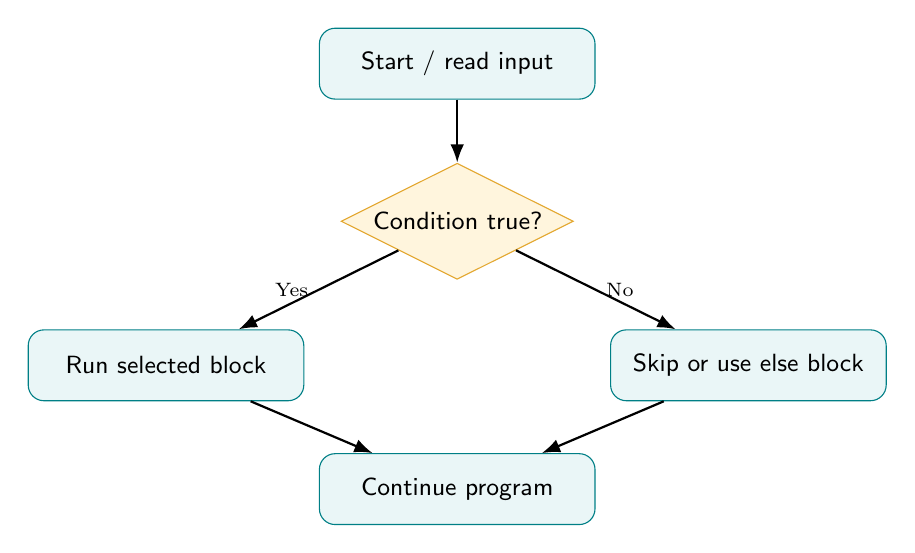
\begin{tikzpicture}[node distance=8mm,every node/.style={font=\small\sffamily,align=center},process/.style={rounded corners=2mm,draw=Teal,fill=Pale,minimum width=35mm,minimum height=9mm},decision/.style={diamond,aspect=2,draw=Gold,fill=LightGold,text width=23mm,inner sep=1pt}]
\node[process] (start) {Start / read input};
\node[decision,below=of start] (test) {Condition true?};
\node[process,below left=10mm and 12mm of test] (yes) {Run selected block};
\node[process,below right=10mm and 12mm of test] (no) {Skip or use else block};
\node[process,below=22mm of test] (end) {Continue program};
\draw[-{Latex},thick] (start)--(test);
\draw[-{Latex},thick] (test)--node[left,font=\scriptsize]{Yes}(yes);
\draw[-{Latex},thick] (test)--node[right,font=\scriptsize]{No}(no);
\draw[-{Latex},thick] (yes)--(end);
\draw[-{Latex},thick] (no)--(end);
\end{tikzpicture}
\end{center}
\textit{Figure 1.1.} A simplified decision flow for a conditional statement.

\section{Functions in Python}
A function is a named, reusable block of code that performs a task. Functions help divide a larger problem into smaller parts, reduce repetition and make a program easier to test. Python includes built-in functions such as \texttt{print()}, \texttt{len()} and \texttt{sum()}; programmers can also define their own functions with \texttt{def}.

\begin{lstlisting}[style=pythonstyle]
def mean(values):
    if len(values) == 0:
        return None
    return sum(values) / len(values)

marks = [72, 81, 67, 90]
print(mean(marks))
\end{lstlisting}
The function accepts a list as an argument and returns its arithmetic mean. The \texttt{return} statement sends a result back to the calling code. Parameters are names in a function definition; arguments are the values supplied when it is called. A local variable created inside a function is normally available only within that function.

\begin{center}
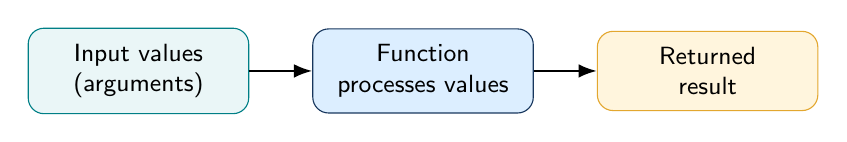
\begin{tikzpicture}[node distance=8mm,every node/.style={font=\small\sffamily,align=center},fbox/.style={rounded corners=2mm,draw=Teal,fill=Pale,minimum width=28mm,minimum height=10mm,inner sep=2mm}]
\node[fbox] (input) {Input values\\(arguments)};
\node[fbox,right=of input,draw=Navy,fill=Sky] (func) {Function\\processes values};
\node[fbox,right=of func,draw=Gold,fill=LightGold] (out) {Returned\\result};
\draw[-{Latex},thick] (input)--(func);
\draw[-{Latex},thick] (func)--(out);
\end{tikzpicture}
\end{center}
\textit{Figure 1.2.} A function receives arguments, performs a task and may return a result.

\subsection{Parameters, return values and scope}
Functions may accept zero or more parameters. A function that returns a value can be used in an expression, while a function that only performs an action may return \texttt{None}. Variables defined inside a function have local scope. Clear names, short functions and appropriate validation improve readability and reliability.

\subsection{Designing a useful function}
A well-designed function usually has one clear responsibility. Its name should describe the task, its parameters should represent the information needed, and its return value should be predictable. Repeating the same calculation in several places makes later changes harder; placing that calculation in one function helps keep results consistent.

\begin{lstlisting}[style=pythonstyle]
def percentage(score, maximum):
    if maximum <= 0:
        raise ValueError("Maximum must be positive")
    return (score / maximum) * 100

print(percentage(45, 50))
\end{lstlisting}
The function checks that the maximum possible score is positive before performing the calculation. This is an example of input validation. In larger programs, functions can be tested with normal values, boundary values and invalid values. A function should also be documented when its purpose or expected inputs are not obvious.

\subsection{Tracing a program step by step}
Tracing means following a program's statements in the order in which they execute and recording how important variables change. It is useful when the output differs from what was expected. Start with the initial values, follow each condition, and update variables only when the relevant statement executes. A small trace table written in a notebook can help beginners reason about loops without relying on guesswork.

Consider a counter that begins at zero and increases once for each item processed. If the update statement is accidentally placed outside the loop, the counter may not represent the number of items. Similarly, changing the order of statements can change the result. Reading the code line by line and testing a small example makes such mistakes easier to identify.

\subsection{Writing readable and maintainable code}
Readable code uses meaningful names, consistent indentation and short blocks that have a clear purpose. A name such as \texttt{total\_marks} communicates more than a single-letter name such as \texttt{x}. Comments should explain the reason for a decision or a non-obvious step rather than repeat every line in English. Blank lines can separate logical parts of a program, but excessive spacing makes a short program harder to follow.

\begin{center}
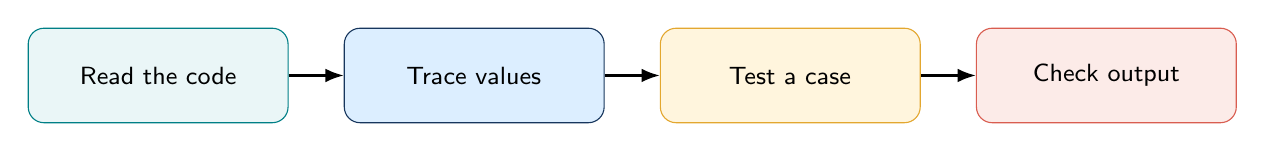
\begin{tikzpicture}[node distance=7mm,every node/.style={font=\small\sffamily,align=center},stage/.style={rounded corners=2mm,draw=Teal,fill=Pale,text width=29mm,minimum height=12mm,inner sep=2mm}]
\node[stage] (read) {Read the code};
\node[stage,right=of read,draw=Navy,fill=Sky] (trace) {Trace values};
\node[stage,right=of trace,draw=Gold,fill=LightGold] (test) {Test a case};
\node[stage,right=of test,draw=Coral,fill=Rose] (check) {Check output};
\draw[-{Latex},thick] (read)--(trace);
\draw[-{Latex},thick] (trace)--(test);
\draw[-{Latex},thick] (test)--(check);
\end{tikzpicture}
\end{center}
\textit{Figure 1.3.} A simple method for tracing and checking a program.

\subsection{Testing with normal, boundary and invalid values}
A normal test checks an expected everyday input. A boundary test checks a value near a limit, such as marks equal to the minimum passing score. An invalid-input test checks what happens when the program receives a negative number where only positive values are permitted, or text where a number is expected. Testing all three kinds of input can reveal problems that one successful example would not show.

For example, a percentage function should be tested with a score of zero, a score equal to the maximum, and a maximum value of zero. The last case should be rejected because division by zero is undefined. Testing does not prove that a program has no defects, but it provides evidence that the program behaves as expected for the cases considered.

\section*{Review Questions}
\begin{enumerate}
\item Distinguish between \texttt{if...else} and \texttt{if...elif...else}.
\item What is the difference between a \texttt{for} loop and a \texttt{while} loop?
\item Write a function that returns the larger of two numbers.
\item Explain why indentation matters in Python.
\end{enumerate}

\chapter{Data Science with NumPy}
\section{Introduction to NumPy}
NumPy is a Python library for numerical computing. Its central data structure is the multidimensional array, commonly called an \texttt{ndarray}. Compared with ordinary Python lists, NumPy arrays support convenient element-wise operations and efficient numerical processing. NumPy is widely used as a foundation for scientific computing and data analysis.

\begin{lstlisting}[style=pythonstyle]
import numpy as np
marks = np.array([72, 81, 67, 90])
print(marks.mean())
print(marks.max())
print(marks.min())
\end{lstlisting}
The import statement makes NumPy available under the short name \texttt{np}, a common convention. The array stores four numerical values. Its methods calculate the mean, maximum and minimum without requiring a manually written loop.

\subsection{Array properties}
The \texttt{ndim} attribute reports the number of dimensions, \texttt{shape} reports the size along each dimension, \texttt{size} gives the total number of elements, and \texttt{dtype} indicates the element data type. A one-dimensional array can represent a sequence; a two-dimensional array can represent rows and columns.

\begin{center}
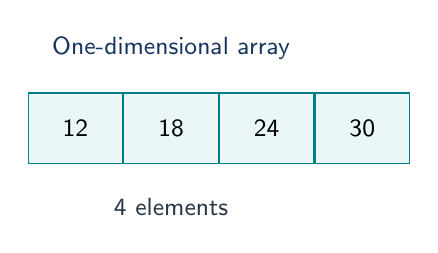
\begin{tikzpicture}[every node/.style={font=\small\sffamily},cell/.style={draw=Teal,fill=Pale,minimum width=12mm,minimum height=9mm}]
\node[cell] (a1) at (0,0) {12};
\node[cell,right=0pt of a1] (a2) {18};
\node[cell,right=0pt of a2] (a3) {24};
\node[cell,right=0pt of a3] (a4) {30};
\node[above=3mm of a2,align=center,text=Navy] {One-dimensional array};
\node[below=3mm of a2,align=center,text=Ink] {4 elements};
\end{tikzpicture}
\end{center}
\textit{Figure 2.2.} A one-dimensional NumPy array stores an ordered sequence of values.

\begin{lstlisting}[style=pythonstyle]
table = np.array([[10, 20, 30],
                  [40, 50, 60]])
print(table.ndim)   # 2
print(table.shape)  # (2, 3)
print(table.size)   # 6
\end{lstlisting}

\section{Array manipulation}
Arrays can be reshaped, joined, split, indexed and sliced. A reshape operation changes the arrangement of elements without changing their total number. Indexing selects particular elements; slicing selects a range. The requested shape must be compatible with the number of values in the array.

\begin{lstlisting}[style=pythonstyle]
values = np.array([1, 2, 3, 4, 5, 6])
matrix = values.reshape(2, 3)
print(matrix)
print(matrix[:, 1])
\end{lstlisting}
The expression \texttt{matrix[:, 1]} selects the second column. In a slice, a colon represents a range along an axis. Understanding array shape is essential when combining data from multiple sources.

\subsection{Indexing and slicing}
NumPy uses zero-based indexing, which means the first element has index 0. Negative indices count from the end of an array. Slicing selects a range using the form \texttt{start:stop:step}; the stop position is excluded. For a two-dimensional array, separate index expressions identify the row and column.

\begin{lstlisting}[style=pythonstyle]
scores = np.array([55, 68, 72, 89, 94])
print(scores[0])       # first value
print(scores[-1])      # last value
print(scores[1:4])     # values at positions 1, 2, 3
print(scores[scores >= 70])
\end{lstlisting}
The last line uses a Boolean condition to select values that are at least 70. Such filtering is useful when exploring measurements, marks or other numerical records. The original data should be preserved when an analysis requires a record of the unmodified values.

\subsection{Broadcasting and practical cautions}
Broadcasting allows NumPy to combine arrays of compatible shapes. For example, adding a single number to an array adds that number to every element. More complex broadcasting follows shape rules, so dimensions should be checked when an operation produces an unexpected result. Arrays should also use appropriate numeric types: converting a decimal measurement to an integer can discard its fractional part.

\subsection{Joining, splitting and copying}
Functions such as \texttt{np.concatenate()} join arrays along a compatible axis. Splitting functions divide arrays into smaller arrays. A view can share underlying data with another array, whereas \texttt{copy()} creates independent data. Changing a shared view may therefore affect the original array.

\section{Array computation}
NumPy supports arithmetic, comparison, logical, statistical and mathematical operations. Many operations are performed element by element. Broadcasting allows arrays with compatible shapes to participate in an operation without manually copying values.

\begin{lstlisting}[style=pythonstyle]
a = np.array([1, 2, 3])
print(a * 2)       # [2 4 6]
print(a + 10)      # [11 12 13]
print(np.sqrt(a))  # square roots
\end{lstlisting}
Common statistical functions include \texttt{sum()}, \texttt{mean()}, \texttt{median()}, \texttt{min()} and \texttt{max()}. Mathematical utilities include trigonometric functions and conversions between degrees and radians. The result type depends on the operation and input types.

\subsection{Why vectorised operations are useful}
A vectorised operation expresses a calculation for an entire array instead of describing each element with a Python loop. This often makes numerical code shorter and can improve performance. The expression should still be chosen for clarity: a compact calculation is not helpful if its meaning is difficult to understand.

For example, if a set of temperatures is stored in an array in degrees Celsius, the conversion to Fahrenheit can be applied to every value using \texttt{temperatures * 9 / 5 + 32}. The formula is applied element by element. Before interpreting a result, check the units, the range of values and whether any missing or unusual measurements need attention.

\begin{center}
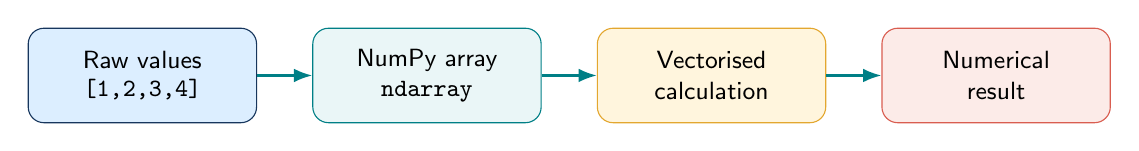
\begin{tikzpicture}[node distance=7mm,every node/.style={font=\small\sffamily,align=center},arr/.style={rounded corners=2mm,draw=Navy,fill=Sky,minimum width=29mm,minimum height=12mm}]
\node[arr] (data) {Raw values\\[-1pt]\texttt{[1,2,3,4]}};
\node[arr,right=of data,fill=Pale,draw=Teal] (array) {NumPy array\\\texttt{ndarray}};
\node[arr,right=of array,fill=LightGold,draw=Gold] (calc) {Vectorised\\calculation};
\node[arr,right=of calc,fill=Rose,draw=Coral] (result) {Numerical\\result};
\draw[-{Latex},thick,Teal] (data)--(array);
\draw[-{Latex},thick,Teal] (array)--(calc);
\draw[-{Latex},thick,Teal] (calc)--(result);
\end{tikzpicture}
\end{center}
\textit{Figure 2.1.} A typical numerical data-processing path.

\subsection{Choosing an array structure}
A one-dimensional array is suitable for a single sequence of measurements, such as daily temperatures. A two-dimensional array can represent a grid or a table of numerical values. Higher-dimensional arrays can represent batches of images or measurements collected across several dimensions. The structure should reflect the meaning of the data, not merely the shape that is convenient to type.

\begin{center}
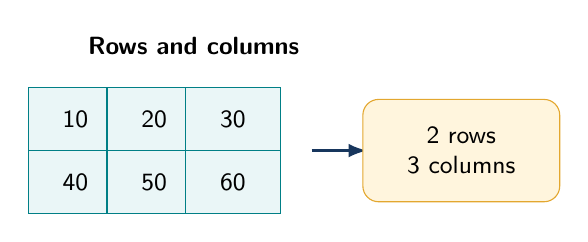
\begin{tikzpicture}[every node/.style={font=\small\sffamily,align=center},cell/.style={draw=Teal,fill=Pale,minimum width=12mm,minimum height=8mm}]
\node[above=2mm] at (1.5,1.1) {\textbf{Rows and columns}};
\foreach \x/\lab in {0/10,1/20,2/30}{\node[cell] at (\x,0.6) {\lab};}
\foreach \x/\lab in {0/40,1/50,2/60}{\node[cell] at (\x,-0.2) {\lab};}
\draw[-{Latex},thick,Navy] (3.0,0.2)--(3.7,0.2);
\node[draw=Gold,fill=LightGold,rounded corners=2mm,minimum width=25mm,minimum height=13mm] at (4.9,0.2) {2 rows\\3 columns};
\end{tikzpicture}
\end{center}
\textit{Figure 2.3.} A two-dimensional array can represent numerical data arranged in rows and columns.

\subsection{Missing values and unusual measurements}
A numerical array can contain values that are mathematically valid but incorrect for the real problem. For instance, a temperature of 900 degrees may be a valid number in a computer but an implausible reading for a classroom thermometer. A negative mark may be outside the permitted range for an examination. Range checks and knowledge of the measurement context help identify such cases.

Missing values require a deliberate decision. If a sensor did not record a reading, replacing it with zero may falsely imply that the measured quantity was zero. Depending on the purpose, the missing value may be excluded from a calculation, investigated, or replaced using a justified method. Always record the choice and consider how it could affect the conclusion.

\subsection{Efficiency and memory}
NumPy is designed for numerical work with arrays and often performs large element-wise calculations more efficiently than manually looping through ordinary Python lists. The actual performance depends on the size of the data, the operation and the computer. For a tiny list, readability matters more than trying to optimise every operation. For large datasets, choosing an appropriate data type and avoiding unnecessary copies can reduce memory use.

\subsection{Practical exercise: summarising measurements}
Create an array containing five fictional daily temperatures. Print the minimum, maximum and mean. Then select values above the mean and explain what the filtered result represents. Change one value to an implausible number and discuss how a range check could identify it. The exercise should include the code, its output and a short interpretation in words.

\section*{Review Questions}
\begin{enumerate}
\item What do \texttt{shape}, \texttt{ndim} and \texttt{dtype} describe?
\item Explain indexing and slicing.
\item What is the difference between a view and a copy?
\item State two advantages of NumPy arrays.
\end{enumerate}

\chapter{Data Analysis}
\section{Introduction to Pandas}
Pandas is an open-source Python library used to organise, clean, analyse and summarise data. It is built around two important data structures: \texttt{Series}, a labelled one-dimensional structure, and \texttt{DataFrame}, a two-dimensional structure with rows and columns. Pandas is useful when data is arranged as a table, such as attendance records, marks, product lists or survey responses.

\begin{lstlisting}[style=pythonstyle]
import pandas as pd
students = pd.DataFrame({
    "Name": ["Asha", "Ravi", "Meena"],
    "Marks": [78, 85, 91],
    "Class": ["X", "X", "X"]
})
print(students)
print(students["Marks"].mean())
\end{lstlisting}
A DataFrame can contain columns of different data types. Column labels help identify fields, while the row index identifies records. Data should be checked for missing values, duplicate records and inconsistent formats before analysis.

\begin{center}
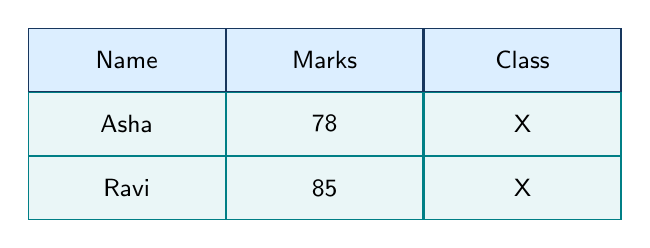
\begin{tikzpicture}[every node/.style={font=\small\sffamily,align=center},head/.style={draw=Navy,fill=Sky,minimum width=25mm,minimum height=8mm},body/.style={draw=Teal,fill=Pale,minimum width=25mm,minimum height=8mm}]
\node[head] (h1) at (0,0) {Name};
\node[head,right=0pt of h1] (h2) {Marks};
\node[head,right=0pt of h2] (h3) {Class};
\node[body,below=0pt of h1] (r11) {Asha};
\node[body,below=0pt of h2] (r12) {78};
\node[body,below=0pt of h3] (r13) {X};
\node[body,below=0pt of r11] (r21) {Ravi};
\node[body,below=0pt of r12] (r22) {85};
\node[body,below=0pt of r13] (r23) {X};
\end{tikzpicture}
\end{center}
\textit{Figure 3.2.} A simplified DataFrame with named columns and individual records.

\section{Working with Series and DataFrames}
A Series stores values with associated labels. A DataFrame groups multiple columns into a table. Pandas can create a Series from a list or dictionary, select columns, filter rows, sort values and calculate summaries.

\begin{lstlisting}[style=pythonstyle]
marks = pd.Series([72, 88, 64, 95])
print(marks.mean())
print(marks[marks >= 80])
\end{lstlisting}
Boolean filtering produces the values that satisfy a condition. In a DataFrame, a similar condition can be used to select records. Labels and positions should not be confused: label-based selection and integer-position selection have different purposes.

\subsection{Selecting, sorting and grouping records}
Pandas makes it possible to select a subset of rows using a condition, sort records by a column and calculate summaries for groups. These operations help turn a large table into information that answers a particular question. A filter should be linked to a clear question, such as identifying records above a chosen threshold.

\begin{lstlisting}[style=pythonstyle]
high_scores = students[students["Marks"] >= 80]
sorted_students = students.sort_values("Marks", ascending=False)
print(high_scores)
print(sorted_students)
\end{lstlisting}
The first expression selects students whose marks are at least 80; the second orders the records from highest marks to lowest. In real projects, the meaning of each column and the unit of measurement should be recorded so that the output is interpreted correctly.

\subsection{Cleaning and summarising data}
Data cleaning may include handling missing values, correcting data types, removing duplicates and standardising text. The correct treatment depends on what a missing or unusual value means in the real context. Deleting records without review can distort the analysis.

A missing value can mean that information was not collected, was not applicable or was accidentally omitted. These situations do not always have the same meaning. Depending on the task, a missing value may be left as missing, investigated with the data owner, or handled using a documented method. Replacing all missing values with zero is not always appropriate because zero may be a valid measurement.

Duplicate records also need careful review. Some duplicates are accidental copies, while others represent legitimate repeated events. Before removing them, check which fields define a unique record. Cleaning decisions should be documented so that another person can understand how the original data was transformed.

\begin{lstlisting}[style=pythonstyle]
print(students.head())
print(students.info())
print(students.isna().sum())
print(students.describe())
\end{lstlisting}
The \texttt{head()} method previews records, \texttt{info()} summarises columns and data types, \texttt{isna().sum()} counts missing values by column, and \texttt{describe()} gives descriptive statistics for suitable columns.

\section{Data visualisation using Matplotlib}
Data visualisation presents information graphically so that patterns, comparisons and changes can be understood. Matplotlib is a Python library for creating charts. The chart type should match the question: bar charts compare categories, line charts show change over an ordered sequence, and scatter plots explore relationships between numerical variables.

\begin{lstlisting}[style=pythonstyle]
import matplotlib.pyplot as plt
subjects = ["English", "Maths", "Science"]
marks = [76, 88, 81]
plt.bar(subjects, marks)
plt.title("Marks by Subject")
plt.xlabel("Subject")
plt.ylabel("Marks")
plt.tight_layout()
plt.show()
\end{lstlisting}
A clear chart needs a meaningful title, labelled axes and a scale that does not mislead. Colours and decorative effects should support interpretation rather than distract from the data. Charts should be checked against the source values before conclusions are drawn.

\subsection{Choosing a chart for the question}
A bar chart is suitable for comparing a small number of categories. A line chart is often appropriate for a measurement recorded over time, such as monthly rainfall. A scatter plot can help reveal whether two numerical variables appear to be related. A histogram shows the distribution of a numerical variable by grouping values into intervals. No chart proves a cause-and-effect relationship by itself.

A chart should include a title that states what is being shown, labels that explain the axes, and units where relevant. The scale should not exaggerate small differences. When comparing groups, use consistent scales and explain any filtering or exclusions. A well-labelled chart helps readers understand both the result and its limits.

\begin{center}
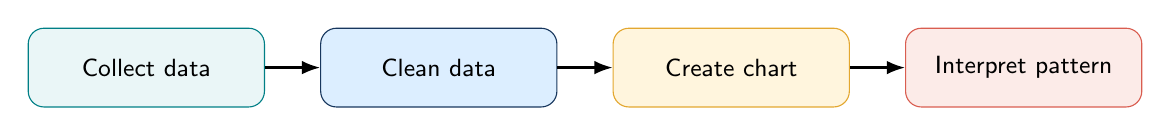
\begin{tikzpicture}[node distance=7mm,every node/.style={font=\small\sffamily,align=center},vbox/.style={rounded corners=2mm,draw=Teal,fill=Pale,minimum width=30mm,minimum height=10mm,inner sep=2mm}]
\node[vbox] (collect) {Collect data};
\node[vbox,right=of collect,draw=Navy,fill=Sky] (clean) {Clean data};
\node[vbox,right=of clean,draw=Gold,fill=LightGold] (visual) {Create chart};
\node[vbox,right=of visual,draw=Coral,fill=Rose] (interpret) {Interpret pattern};
\draw[-{Latex},thick] (collect)--(clean);
\draw[-{Latex},thick] (clean)--(visual);
\draw[-{Latex},thick] (visual)--(interpret);
\end{tikzpicture}
\end{center}
\textit{Figure 3.3.} A simple sequence for producing a trustworthy data visualisation.

\begin{center}
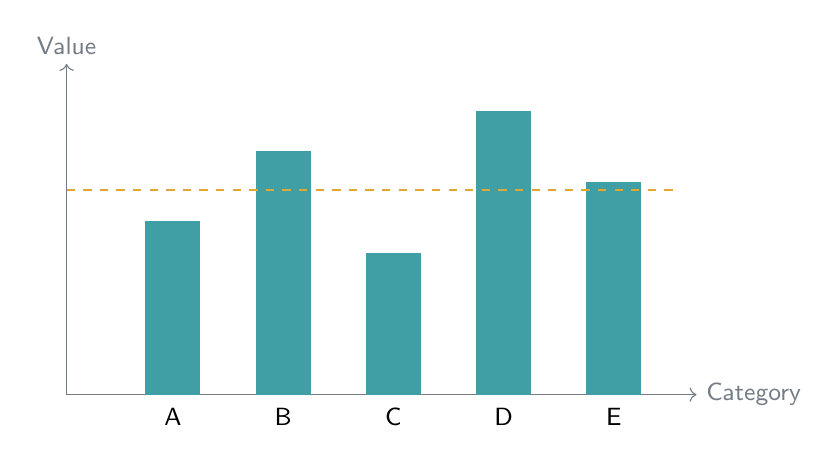
\begin{tikzpicture}[every node/.style={font=\small\sffamily}]
\draw[Ink!65,->] (0,0)--(8,0) node[right]{Category};
\draw[Ink!65,->] (0,0)--(0,4.2) node[above]{Value};
\foreach \x/\h/\lab in {1/2.2/A,2.4/3.1/B,3.8/1.8/C,5.2/3.6/D,6.6/2.7/E}{
\fill[Teal!75] (\x,0) rectangle +(0.7,\h);
\node[below] at (\x+0.35,-.05) {\lab};
}
\draw[Gold,dashed] (0,2.6)--(7.8,2.6);
\end{tikzpicture}
\end{center}
\textit{Figure 3.1.} A schematic bar chart showing how categories can be compared.

\subsection{Understanding records and data types}
A data table represents observations as rows and properties as columns. In a student marks dataset, one row may represent one learner and columns may represent a name, subject, marks and examination date. A column should have a consistent meaning. If marks are stored partly as numbers and partly as text, calculations and comparisons may behave unexpectedly.

A Pandas Series is a one-dimensional labelled structure. A DataFrame combines rows and columns and can contain columns with different data types. The index labels rows, while column names identify fields. An index is not necessarily a unique identity for a real-world person or item; if a reliable identifier is required, it should be designed and checked separately.

\subsection{Filtering records carefully}
Filtering selects records that satisfy a condition. Multiple conditions can be combined, but each condition should be enclosed in parentheses when using Pandas Boolean expressions. The symbols \texttt{\&} and \texttt{|} represent element-wise AND and OR; Python's \texttt{and} and \texttt{or} are not substitutes for these operators in a Series expression.

\begin{lstlisting}[style=pythonstyle]
import pandas as pd

students = pd.DataFrame({
    "Name": ["Asha", "Ravi", "Meena", "Imran"],
    "Marks": [78, 91, 84, 65],
    "Present": [True, True, False, True]
})
high = students[students["Marks"] >= 80]
print(high[["Name", "Marks"]])
\end{lstlisting}
The expression creates a smaller DataFrame containing only records with marks of at least 80, and then displays selected columns. In a real report, the filter condition should be stated clearly so readers understand which records were included.

\subsection{Grouping and summarising}
Grouping is useful when the question asks for a summary by category, such as average marks by subject or the number of records in each region. A group summary can hide differences between individual observations, so it should be interpreted at the correct level. When group sizes differ, a total and an average answer different questions; choose the statistic that fits the purpose.

\subsection{Reproducible data cleaning}
A reproducible cleaning process records what was changed and why. Keep an untouched copy of the original data where appropriate, and perform cleaning steps in a clear order. Check the number of rows before and after removing duplicates, confirm that conversions succeeded, and inspect a sample of the cleaned result. These checks reduce the risk of silently removing valid records or introducing errors.

\begin{center}
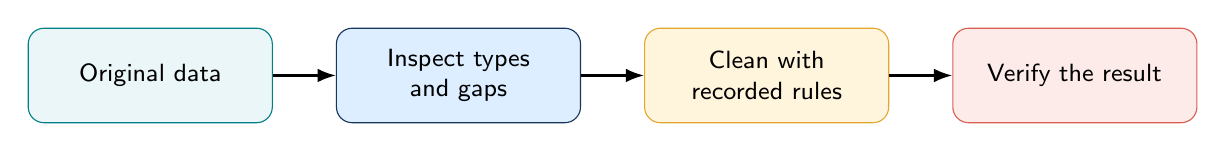
\begin{tikzpicture}[node distance=8mm,every node/.style={font=\small\sffamily,align=center},dbox/.style={rounded corners=2mm,draw=Teal,fill=Pale,text width=27mm,minimum height=12mm,inner sep=2mm}]
\node[dbox] (source) {Original data};
\node[dbox,right=of source,draw=Navy,fill=Sky] (inspect) {Inspect types and gaps};
\node[dbox,right=of inspect,draw=Gold,fill=LightGold] (clean) {Clean with recorded rules};
\node[dbox,right=of clean,draw=Coral,fill=Rose] (verify) {Verify the result};
\draw[-{Latex},thick] (source)--(inspect);
\draw[-{Latex},thick] (inspect)--(clean);
\draw[-{Latex},thick] (clean)--(verify);
\end{tikzpicture}
\end{center}
\textit{Figure 3.4.} A repeatable workflow for preparing tabular data.

\section*{Review Questions}
\begin{enumerate}
\item Differentiate between a Series and a DataFrame.
\item Why is data cleaning necessary?
\item Name four useful Pandas methods.
\item Choose an appropriate chart to compare marks in several subjects and explain why.
\end{enumerate}

\chapter{Neural Networks and Machine Learning Tools}
\section{Artificial Neural Networks}
An Artificial Neural Network (ANN) is a computational model inspired in a broad way by networks of connected neurons. In a typical neural network, units receive numerical inputs, apply weights and a bias, pass the result through an activation function, and send outputs to the next layer. Networks can learn patterns by adjusting parameters during training.

\begin{center}
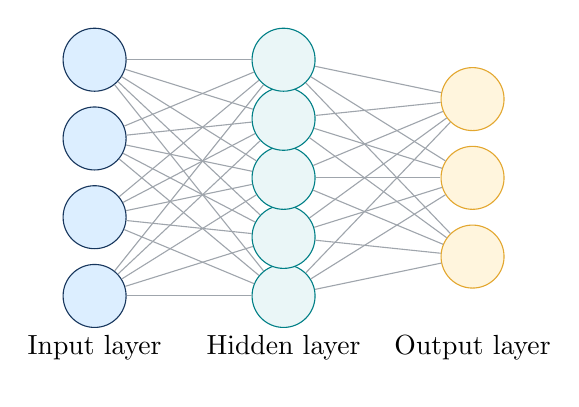
\begin{tikzpicture}[x=1cm,y=1cm,every node/.style={circle,draw=Navy,fill=Sky,minimum size=8mm,inner sep=0pt},>=Latex]
\foreach \y/\id in {0/A,1/B,2/C,3/D}{\node (i\id) at (0,\y) {};}
\foreach \y/\id in {0/A,0.75/B,1.5/C,2.25/D,3/E}{\node[fill=Pale,draw=Teal] (h\id) at (2.4,\y) {};}
\foreach \y/\id in {0.5/A,1.5/B,2.5/C}{\node[fill=LightGold,draw=Gold] (o\id) at (4.8,\y) {};}
\foreach \i in {A,B,C,D}{\foreach \h in {A,B,C,D,E}{\draw[Ink!45] (i\i)--(h\h);}}
\foreach \h in {A,B,C,D,E}{\foreach \o in {A,B,C}{\draw[Ink!45] (h\h)--(o\o);}}
\node[draw=none,fill=none,rectangle] at (0,-.65) {Input layer};
\node[draw=none,fill=none,rectangle] at (2.4,-.65) {Hidden layer};
\node[draw=none,fill=none,rectangle] at (4.8,-.65) {Output layer};
\end{tikzpicture}
\end{center}
\textit{Figure 4.1.} A simplified fully connected neural network. The drawing is conceptual; real networks can contain many layers and different connection patterns.

\subsection{Training and prediction}
During training, a network processes examples and compares its output with the expected target. A loss function measures the difference, and an optimisation method adjusts model parameters to reduce that loss. After training, the model can make predictions on new inputs. Performance on training examples alone is not enough; evaluation on separate data helps estimate how well the model generalises.

\subsection{Weights, activation functions and loss}
A weight controls how strongly an input contributes to a unit's calculation. A bias shifts the calculation, and an activation function transforms the result. Common activation functions include ReLU for many hidden layers and sigmoid for some binary-output tasks. The choice depends on the model design and the problem being solved.

A loss function measures how far a model's predictions are from the expected targets during training. The training process adjusts weights and biases to reduce the loss. A lower training loss does not automatically mean that a model will perform well on unfamiliar examples, so evaluation must use data that was not used to fit the model.

\subsection{Overfitting and generalisation}
Overfitting occurs when a model learns details or noise specific to its training examples and performs poorly on new data. A model that is too simple may also fail to capture useful patterns; this is often described as underfitting. Careful data splitting, suitable model complexity and evaluation on representative examples help assess generalisation. The test set should not be repeatedly used to tune every decision, because that can make the final estimate overly optimistic.

\section{Applications of neural networks}
Neural networks are used in image and speech recognition, handwriting recognition, language processing, recommendation systems, forecasting and selected healthcare applications. Face recognition can support device authentication; speech-to-text systems convert spoken language into text; recommendation systems rank items that may interest a user. Such applications can make errors, so human review and suitable safeguards remain important, especially in high-impact settings.

\subsection{Responsible use}
Data quality, privacy, fairness and transparency affect the reliability of an AI application. A model trained on unrepresentative examples may perform poorly for some groups. Sensitive personal data should be handled carefully, and a prediction should not automatically be treated as a fact. The system's purpose, limitations and evaluation results should be documented.

\subsection{Privacy, fairness and human oversight}
Responsible AI development begins with asking whether the data is needed and whether it may be used for the intended purpose. Personal details should not be collected simply because they are available. Access should be limited, files should be protected, and information should not be shared without appropriate permission.

Fairness requires checking whether the examples represent the people and situations in which the system will be used. An error can affect groups differently, especially when the training data is incomplete or unbalanced. A responsible project explains known limitations and provides a way for a person to review important decisions. AI outputs should be treated as information to assess, not as unquestionable truth.

\section{Machine learning tools}
Python's data-science ecosystem includes tools for different stages of an AI workflow. NumPy supports numerical arrays; Pandas supports tabular data handling; Matplotlib supports visualisation; Scikit-learn provides common machine-learning algorithms and evaluation utilities; TensorFlow and Keras support the development of neural-network models; XGBoost provides optimised gradient-boosting methods.

\begin{center}
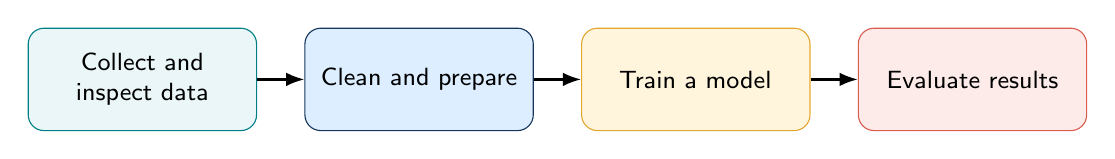
\begin{tikzpicture}[node distance=6mm,every node/.style={font=\small\sffamily,align=center},mlstage/.style={rounded corners=2mm,draw=Teal,fill=Pale,text width=25mm,minimum height=13mm,inner sep=2mm}]
\node[mlstage] (data) {Collect and inspect data};
\node[mlstage,right=of data,draw=Navy,fill=Sky] (clean) {Clean and prepare};
\node[mlstage,right=of clean,draw=Gold,fill=LightGold] (train) {Train a model};
\node[mlstage,right=of train,draw=Coral,fill=Rose] (eval) {Evaluate results};
\draw[-{Latex},thick] (data)--(clean);
\draw[-{Latex},thick] (clean)--(train);
\draw[-{Latex},thick] (train)--(eval);
\end{tikzpicture}
\end{center}
\textit{Figure 4.2.} A simplified machine-learning workflow.

\subsection{How a neural network makes a prediction}
A neural network transforms input values through a series of connected calculations. In a simple unit, inputs are multiplied by weights, combined with a bias and passed through an activation function. The output of one layer becomes the input to the next layer. During training, the model adjusts its parameters using examples and a learning procedure.

\begin{center}
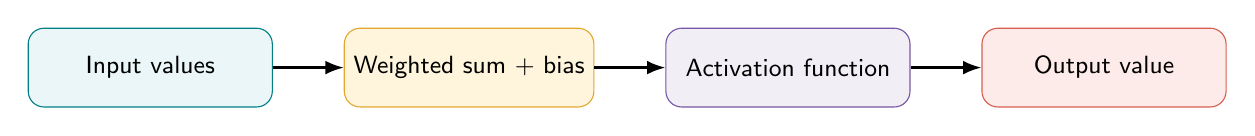
\begin{tikzpicture}[node distance=9mm,every node/.style={font=\small\sffamily,align=center},unit/.style={circle,draw=Navy,fill=Sky,minimum size=8mm,inner sep=0pt},calc/.style={rounded corners=2mm,draw=Teal,fill=Pale,minimum width=31mm,minimum height=10mm}]
\node[calc] (input) {Input values};
\node[calc,right=of input,draw=Gold,fill=LightGold] (weighted) {Weighted sum + bias};
\node[calc,right=of weighted,draw=Violet,fill=Violet!10] (activation) {Activation function};
\node[calc,right=of activation,draw=Coral,fill=Rose] (output) {Output value};
\draw[-{Latex},thick] (input)--(weighted);
\draw[-{Latex},thick] (weighted)--(activation);
\draw[-{Latex},thick] (activation)--(output);
\end{tikzpicture}
\end{center}
\textit{Figure 4.3.} A simplified view of the calculation performed by a neural-network unit.

\subsection{Training, validation and testing}
A dataset is often divided into separate parts for training, validation and testing. Training examples are used to fit model parameters. Validation examples help compare model settings during development. Test examples are held aside for a final evaluation after important choices have been made. The exact split depends on the amount and structure of the available data, and time-based data may require a time-aware split.

If examples from the same person or event appear in both training and test sets, the test result may be overly optimistic. This is a form of data leakage. Data preparation steps such as scaling should also be fitted using training data only and then applied consistently to validation and test data. A fair evaluation depends on keeping information from the test set out of the training process.

\subsection{Classification and regression}
Classification predicts a category, such as whether an image contains a cat or a dog. Regression predicts a numerical value, such as an estimated temperature. Accuracy can be useful for some classification tasks, but it may be misleading when one category is much more common than another. Precision and recall can provide additional information when false positives and false negatives have different consequences.

For regression, measures such as mean absolute error describe the typical size of prediction errors in the units of the target. The chosen measure should be explained in plain language. A model should also be compared with a simple baseline, such as always predicting the average, to check whether the more complex method adds value.

\subsection{Limitations of neural networks}
Neural networks may require substantial data and computing resources, and their behaviour can be difficult to explain. They can reproduce patterns and biases in training data. A high score on one dataset does not guarantee the same performance in a different school, region, language or time period. Monitoring, human review and clear limits on use are important where mistakes could affect people.

\subsection{Practical comparison exercise}
Imagine a system that predicts whether a learner may need additional help based on practice quiz results. Discuss what the inputs might be, which information should not be collected, and how the system could be checked for errors. Explain why a teacher should review the context before acting on a prediction. The goal is to evaluate responsible design, not to label any real learner.

\section*{Review Questions}
\begin{enumerate}
\item Name the main layers in a simple ANN.
\item What is the purpose of a loss function?
\item Give three applications of neural networks.
\item Match NumPy, Pandas, Matplotlib and Scikit-learn with their common uses.
\item Why should a model be evaluated on data not used for training?
\end{enumerate}

\chapter{AI Project}
\section{Project guidelines}
An AI project begins with a clear problem rather than with a tool. The problem statement should explain who experiences the problem, why it matters and what a useful result would look like. A manageable project has a defined scope, accessible data, a realistic schedule and criteria for evaluating the result.

\subsection{A practical project cycle}
A typical project cycle includes identifying a problem, defining the objective, collecting or selecting data, understanding and preparing the data, choosing an approach, building a prototype, testing it, evaluating outcomes and presenting findings. The stages may be revisited when testing reveals an issue.

\begin{center}
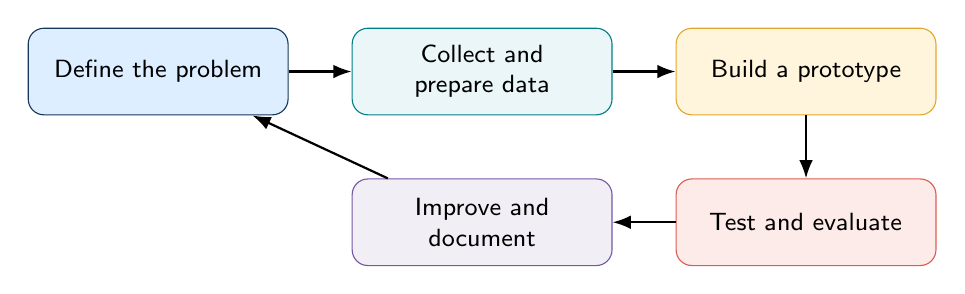
\begin{tikzpicture}[node distance=8mm,every node/.style={font=\small\sffamily,align=center},p/.style={rounded corners=2mm,draw=Navy,fill=Sky,text width=29mm,minimum height=11mm,inner sep=2mm}]
\node[p] (problem) {Define the problem};
\node[p,right=of problem,draw=Teal,fill=Pale] (data) {Collect and prepare data};
\node[p,right=of data,draw=Gold,fill=LightGold] (build) {Build a prototype};
\node[p,below=of build,draw=Coral,fill=Rose] (test) {Test and evaluate};
\node[p,left=of test,draw=Violet,fill=Violet!10] (improve) {Improve and document};
\draw[-{Latex},thick] (problem)--(data);
\draw[-{Latex},thick] (data)--(build);
\draw[-{Latex},thick] (build)--(test);
\draw[-{Latex},thick] (test)--(improve);
\draw[-{Latex},thick] (improve)--(problem);
\end{tikzpicture}
\end{center}
\textit{Figure 5.1.} An iterative project cycle. Evaluation may lead to improvements or a revised problem definition.

\section{Project formats and documentation}
A project report should communicate the problem, objective, data source, method, implementation, evaluation, limitations and conclusion. Include diagrams or tables when they make the method easier to understand. Code should be organised, named clearly and accompanied by instructions for running it. Data sources and external materials should be acknowledged.

\subsection{Choosing evaluation measures}
The measure depends on the task. A classification project may report accuracy and, where appropriate, precision, recall and a confusion matrix. A numerical prediction task may use an error measure such as mean absolute error. A visualisation project should be assessed for correctness, readability and whether it answers the original question. A single score rarely tells the whole story.

\section{Project review}
A useful review considers whether the project solves the stated problem, whether the data and method are appropriate, whether the result can be reproduced, and whether limitations are acknowledged. Reviewers should consider privacy, possible bias, safety and the consequences of incorrect predictions. Clear documentation makes the project easier to understand and maintain.

\begin{center}
\begin{tabularx}{\textwidth}{>{\bfseries}p{.25\textwidth}X}
\toprule
Review area & Questions to consider\\
\midrule
Problem and scope & Is the objective clear and achievable?\\
Data & Are the source, quality, permissions and limitations recorded?\\
Method & Is the selected approach suitable for the task?\\
Evaluation & Are the measures relevant and the results honestly reported?\\
Responsible use & Have privacy, bias and potential harm been considered?\\
Documentation & Can another person understand and reproduce the work?\\
\bottomrule
\end{tabularx}
\end{center}

\section{Sample project: student marks analysis}
A small marks-analysis project is a useful example of a data-focused AI learning task. A learner can create a table of fictional student marks, inspect the values with Pandas, calculate summaries with NumPy and present subject comparisons using Matplotlib. This project demonstrates data handling and communication; it should not be described as an AI prediction model unless a learning method is actually implemented and evaluated.

\begin{lstlisting}[style=pythonstyle]
import pandas as pd
import matplotlib.pyplot as plt

data = pd.DataFrame({
    "Subject": ["English", "Maths", "Science"],
    "Marks": [76, 88, 81]
})
print("Average:", data["Marks"].mean())
plt.bar(data["Subject"], data["Marks"])
plt.title("Sample Marks by Subject")
plt.ylabel("Marks")
plt.tight_layout()
plt.show()
\end{lstlisting}
The values are illustrative, not real student records. A report should describe the data, explain each step, include the chart, note limitations and avoid identifying real learners without a valid reason and appropriate permission.

\subsection{Planning the work and presenting results}
Before writing code, prepare a short plan with the project objective, required inputs, expected outputs and a list of tasks. Divide the work into manageable steps, such as preparing a data file, checking its quality, performing calculations, creating a chart and writing a conclusion. A small prototype should be tested early so that major problems are discovered before the final report is prepared.

The final presentation should explain the original question, the approach used and the evidence that supports the conclusion. Screenshots or diagrams can help readers follow the process, but they should be relevant and clearly labelled. If the result is uncertain or the dataset is small, state that limitation rather than making a broader claim than the evidence supports. Keep a copy of the code and note the software libraries required to run it.

\subsection{Defining a measurable project objective}
A good objective describes the problem, the intended user and the result that would count as useful. “Use AI to improve education” is too broad to guide a small project. “Create a chart that compares fictional marks across three subjects and explain the highest and lowest values” is specific and can be completed with a small dataset. If the project claims to predict an outcome, the report must explain how the prediction is trained and evaluated.

Before selecting a tool, ask whether AI is necessary. A clear set of rules or a simple chart may solve the problem more transparently than a machine-learning model. The best project is not necessarily the one with the most complex technology; it is the one that addresses the stated need safely and convincingly.

\subsection{Data permissions and documentation}
Use data that is permitted for the project. For classroom practice, fictional or appropriately anonymised examples are often sufficient. Do not upload personal records to online services unless there is a valid reason and appropriate permission. Keep track of the data source, collection date, fields, units, cleaning decisions and known limitations. If external code or images are used, acknowledge the source and respect its licence.

\subsection{A practical project schedule}
Divide a project into small tasks: define the question, prepare data, implement the method, test the result, create a visual explanation and write the report. Set a completion check for each task. Keep the scope realistic so that enough time remains for testing and documenting the work. If a step takes longer than expected, simplify optional features rather than skipping evaluation.

\subsection{Interpreting results honestly}
A result should be described in proportion to the evidence. A small sample may illustrate a method but cannot represent every learner or community. A correlation between two measurements does not prove that one causes the other. If the output changes substantially when one data point is removed, mention that sensitivity. Include failures and limitations as part of the report, not as details to hide.

\subsection{Project report structure}
A useful report can contain a title, problem statement, objective, data description, method, tools, implementation steps, results, evaluation, limitations, responsible-use considerations and conclusion. Each section should help the reader understand a different part of the work. Diagrams should be labelled, code should be formatted clearly, and every figure should be discussed in the text. A conclusion should answer the original question and avoid claims that were not tested.

\begin{center}
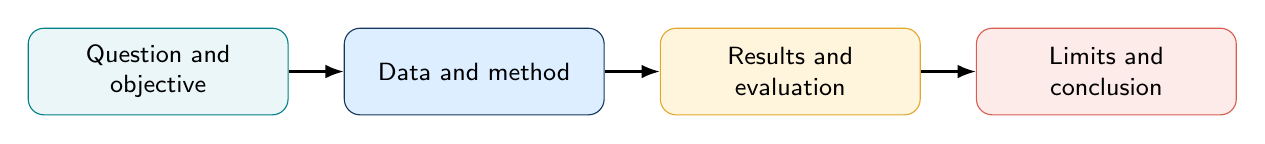
\begin{tikzpicture}[node distance=7mm,every node/.style={font=\small\sffamily,align=center},report/.style={rounded corners=2mm,draw=Teal,fill=Pale,text width=29mm,minimum height=11mm,inner sep=2mm}]
\node[report] (question) {Question and objective};
\node[report,right=of question,draw=Navy,fill=Sky] (data) {Data and method};
\node[report,right=of data,draw=Gold,fill=LightGold] (result) {Results and evaluation};
\node[report,right=of result,draw=Coral,fill=Rose] (limits) {Limits and conclusion};
\draw[-{Latex},thick] (question)--(data);
\draw[-{Latex},thick] (data)--(result);
\draw[-{Latex},thick] (result)--(limits);
\end{tikzpicture}
\end{center}
\textit{Figure 5.2.} A logical structure for explaining an AI project.

\subsection{Reflection after completion}
After completing the project, review whether the original objective was met, what evidence supports the result and which steps were difficult. Identify one improvement that would make the result more reliable or easier to use. A useful reflection is specific: it describes what happened and what would be changed next time, rather than simply saying that the project was good or bad.

\section*{Review Questions}
\begin{enumerate}
\item List the major stages of an AI project.
\item Why is the problem statement important?
\item What should a project report contain?
\item Explain why evaluation measures depend on the task.
\item Identify two privacy or fairness questions to consider before using data.
\end{enumerate}

\end{document}
